\chapter{Speech Presence Probability Implementation}

In this chapter it will be shown how the SPP method found in \cite{Gerkmann2011NoisePresence} can be implemented in Matlab so that the different variations in the algorithm can be tested later.

\begin{figure}[!ht]
  \centering
	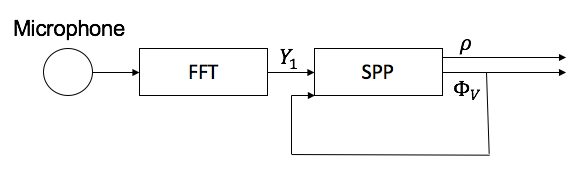
\includegraphics[width=100mm]{Kap3/SPPdiag}
	\caption{Block diagram of SPP method.}
	\label{fig:SPPdiag}
\end{figure}

\section{Implementation}

Under the assumption that a soft decision VAD might be more precise than the hard decision, the following algorithm will be included in the  multi-channel noise reduction method.  Following this, the SPP was found as proposed in \cite{Gerkmann2011NoisePresence}: 

\begin{equation}\label{SPP}
{\rho=\frac{1}{\left( 1+(1+\xi_{opt})exp\left(-\frac{|Y_1(k,n)|^2}{\Phi_{V}(k,n-1)}\frac{\xi_{opt}}{\xi_{opt}+1}\right)\right)}}
\end{equation}


Where $\rho$ is the variable that takes values between 0 and 1 indicating the probability of voice presence (0 means no voice, 1 means total certitude of voice) and  $\xi_{opt}$ is a fixed a priori SNR, $Y_1$ is the input , $\Phi_V$ is the noise power density, and:

\begin{equation}
\Phi_{V,SPP}(k,n)=\rho \Phi_{V,SPP}(k,n-1)+(1-\rho)|Y_1(k,n)|^2
\label{psdNoi}
\end{equation}


After this, the value of $\Phi_{N,SPP}$ is integrated to the estimated noise power density:

\begin{equation}
\Phi_{V}(k,n)=\alpha_{N,SPP} \Phi_{V}(k,n-1)+(1-\alpha_{N,SPP})\Phi_{V,SPP}(k,n)
\label{noipsdc}
\end{equation}

In \cite{PeiCheeYongSvenNordholm2012NoiseSmoothong} it is proposed a similar method in which the value of $\rho$ is modeled as a sigmoid function, with this, it is possible to adjust its slope ($a_{sig}$)  and mean ($c_{sig}$). The value of $\rho$ wil be given as:

\begin{equation}\label{SPPyong}
{\rho=\frac{1}{\left( 1+exp\left(-a_{sig}\left(\frac{|Y_1(k,n)|^2}{\Phi_{V}(k,n-1)}-c_{sig}\right)\right)\right)}}
\end{equation}


where:

$$a_{sig}=\frac{\xi_{opt}}{\xi_{opt}+1}$$
$$c_{sig}=log\left(\frac{P(\mathpzc{H}_0)}{P(\mathpzc{H}_1}(1-\xi_{opt}) \right)\frac{\xi_{opt}+1}{\xi_{opt}}$$

In this project both SPP methods will be tested and compared when they are used with as part of the MWF noise reduction method.

\section{Stagnation}

This algorithms give a very close estimation of the ideal SPP, but, it is susceptible to have stagnation problems. It can be seen that if the spectral noise power is underestimated, in equation \eqref{SPP}, it may lead to $\rho=1$ even if the power of the input is low with respect to the real and unknown noise power. In this case the equation \eqref{psdNoi} won't update the noise power anymore and the noise will remain underestimated. This is know as stagnation.

Both described  methods also propose a way to avoid stagnation which will be explained in this chapter and part of the testing algorithms.

\subsubsection{Tracking Time Average}

The algorithm showed in \cite{Gerkmann2011NoisePresence} propose to force a lower the value of $\rho$ when it's time average is higher than certain threshold. This means, if $\rho$ has high values for too long it's forced to a lower one, this can be expressed as:


\begin{equation}\label{Stag1}
\rho = \left\{
\begin{array}{c l}
 min(0.5 , \rho) &  \bar{\rho}>0.9\\
 \rho & else
\end{array}
\right.
\end{equation}

\subsubsection{3 Regions}

In \cite{PeiCheeYongSvenNordholm2012NoiseSmoothong}, the SPP was categorized in three regions which control the update speed of the noise PSD  estimate from equation \ref{noipsdc} as follows:
 
\begin{equation}\label{Stag2}
\tau= \left\{ \begin{array}{lcc}
             \mathpzc{P}_1 &   if  & \rho \leq 0.3 \\
             \\ \mathpzc{P}_2 &  if & 0.3 < \rho < 0.6 \\
             \\ min(\mathpzc{P}_3,\rho) &  if  &\rho \geq 0.6
             \end{array}
   \right.
\end{equation}
 \medskip
 
 After, finding the right $\tau$, the smoothing value $\alpha$ is found with the following equation:
 
\begin{equation}
C(\tau_m)=\alpha =  e^{\frac{-2.2R}{F_{s}*\tau}}
\label{fromTime}
\end{equation}


The proposed time values for $\mathpzc{P}_i$ are:

$$\mathpzc{P}_1=50ms$$
$$\mathpzc{P}_2=80ms$$
$$\mathpzc{P}_3=240ms$$







